% chapters/04_results.tex
% Presents the quantitative and qualitative findings of the study.
% FIX: Corrected pgfplots syntax to handle special characters in labels.
% FIX: Restored the third figure which was accidentally deleted.

\chapter{Data Presentation and Analysis}
\label{chap:results}

This chapter presents the findings of the study based on quantitative household survey data, qualitative interviews with key informants, and field observations at the Beadu solid waste disposal site. The analysis highlights socio-demographic characteristics, prevalence of reported health problems, waste management practices, perceived health impacts, and community awareness.

\section{Socio-Demographic Characteristics of Respondents}

A total of 150 households were surveyed. Table~\ref{tab:demographics} summarizes the socio-demographic characteristics of the respondents. The majority of respondents were female (64.7\%), reflecting their central role in household management and caregiving. The dominant age group was 31--45 years (43.3\%). Educational attainment was low, with 60\% of respondents having no formal or only primary education. Regarding occupation, informal employment (36.7\%) and unemployment (26.7\%) were most common. Nearly half of respondents (46.7\%) lived within 500 meters of the Beadu site, indicating high potential exposure.

\begin{table}[h!]
\centering
\caption{Socio-Demographic Characteristics of Surveyed Households (N=150)}
\label{tab:demographics}
\begin{tabular}{@{}llcc@{}}
\toprule
\textbf{Characteristic} & \textbf{Category} & \textbf{Frequency (n)} & \textbf{Percentage (\%)} \\ \midrule
Gender of Respondent & Male & 53 & 35.3 \\
                     & Female & 97 & 64.7 \\ \midrule
Age Group (Years)    & 18--30 & 30 & 20.0 \\
                     & 31--45 & 65 & 43.3 \\
                     & 46--60 & 40 & 26.7 \\
                     & >60    & 15 & 10.0 \\ \midrule
Education Level       & No formal education & 45 & 30.0 \\
                      & Primary education    & 45 & 30.0 \\
                      & Secondary education  & 35 & 23.3 \\
                      & Tertiary education   & 25 & 16.7 \\ \midrule
Occupation            & Employed (Formal)    & 30 & 20.0 \\
                      & Employed (Informal)  & 55 & 36.7 \\
                      & Unemployed           & 40 & 26.7 \\
                      & Housewife/Student/Other & 25 & 16.7 \\ \midrule
Distance from Site & <500 meters & 70 & 46.7 \\
                   & 500m--1 km  & 80 & 53.3 \\ \bottomrule
\end{tabular}
\end{table}


\section{Prevalence of Reported Health Conditions}

Respondents reported a range of health problems over the previous six months. The most frequently reported conditions were acute respiratory infections (63.3\%), diarrheal diseases (53.3\%), and skin irritations (46.7\%). Table~\ref{tab:health} and Figure~\ref{fig:healthproblems} present the distribution.

\begin{table}[h!]
\centering
\caption{Self-reported health problems among surveyed households (N=150).}
\label{tab:health}
\begin{tabular}{@{}lcc@{}}
\toprule
\textbf{Health Problem} & \textbf{n} & \textbf{Percentage (\%)} \\ 
\midrule
Acute Respiratory Infections (ARIs) & 95 & 63.3 \\
Diarrheal Diseases                   & 80 & 53.3 \\
Skin Rashes/Irritations              & 70 & 46.7 \\
Eye Irritations                      & 55 & 36.7 \\
Malaria/Vector-borne Diseases        & 30 & 20.0 \\
Other (e.g., headaches, nausea)      & 25 & 16.7 \\
\bottomrule
\end{tabular}
\end{table}

\begin{figure}[h!]
\centering
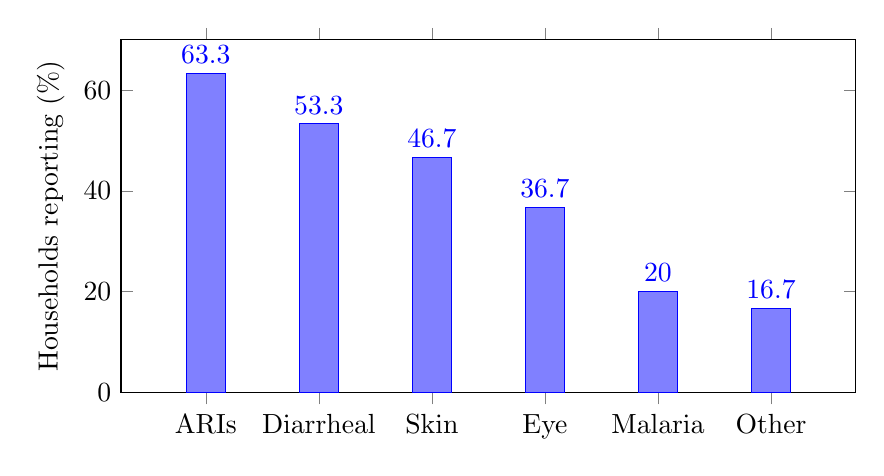
\begin{tikzpicture}
\begin{axis}[
    ybar,
    bar width=14pt,
    width=0.9\textwidth,
    height=0.5\textwidth,
    ymin=0,
    ymax=70,
    ylabel={Households reporting (\%)},
    symbolic x coords={ARIs, Diarrheal, Skin, Eye, Malaria, Other},
    xtick=data,
    nodes near coords,
    nodes near coords align={vertical},
    enlarge x limits=0.15,
]
\addplot+[fill=blue!50] coordinates {(ARIs,63.3) (Diarrheal,53.3) (Skin,46.7) (Eye,36.7) (Malaria,20.0) (Other,16.7)};
\end{axis}
\end{tikzpicture}
\caption{Prevalence of self-reported health problems among households.}
\label{fig:healthproblems}
\end{figure}


\section{Association Between Proximity and Reported Illnesses}

A chi-square test revealed a statistically significant association between proximity to the Beadu site and perceived health problems ($\chi^2(1)=5.21, p<0.05$). Table~\ref{tab:proximity} shows that households closer to the site (<500 meters) were far more likely (92.9\%) to link their illnesses to the dumpsite than those living farther away. This is visualized in Figure~\ref{fig:proximity}.

\begin{table}[h!]
\centering
\caption{Perceived link between proximity to site and health problems (N=150).}
\label{tab:proximity}
\begin{tabular}{@{}lccc@{}}
\toprule
\textbf{Proximity to Site} & \textbf{Yes (n,\%)} & \textbf{No (n,\%)} & \textbf{Total} \\ 
\midrule
< 500 meters   & 65 (92.9) & 5 (7.1)   & 70 \\
500m--1 km     & 63 (78.8) & 17 (21.2) & 80 \\
\midrule
Total          & 128 (85.3) & 22 (14.7) & 150 \\
\bottomrule
\end{tabular}
\end{table}

\begin{figure}[h!]
\centering
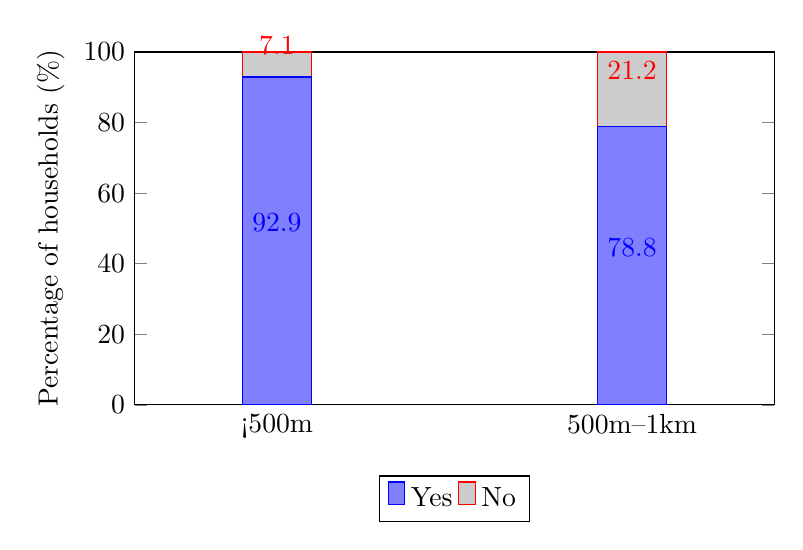
\begin{tikzpicture}
\begin{axis}[
    ybar stacked,
    bar width=25pt,
    width=0.8\textwidth,
    height=0.5\textwidth,
    ymin=0,
    ymax=100,
    ylabel={Percentage of households (\%)},
    symbolic x coords={groupA, groupB}, % Use simple internal names
    xtick=data,
    xticklabels={<500m, 500m--1km}, % Provide the display text here
    nodes near coords,
    nodes near coords align={vertical},
    enlarge x limits=0.4,
    legend style={at={(0.5,-0.2)},anchor=north,legend columns=-1},
]
\addplot+[fill=blue!50] coordinates {(groupA,92.9) (groupB,78.8)};
\addplot+[fill=gray!40] coordinates {(groupA,7.1) (groupB,21.2)};
\legend{Yes, No}
\end{axis}
\end{tikzpicture}
\caption{Perceived link between proximity to site and health problems.}
\label{fig:proximity}
\end{figure}


\section{Community Awareness and Attitudes}

Awareness of health risks was generally high (78\% of respondents agreed that improper waste disposal causes illness). However, satisfaction with municipal waste services was very low (78\% disagreed that services were adequate). While 45\% expressed willingness to pay for improved services, actual segregation practices remained minimal (only 25\% practiced separation at home). Table~\ref{tab:awareness} and Figure~\ref{fig:awareness} summarize these attitudes.

\begin{table}[h!]
\centering
\caption{Community awareness and attitudes towards solid waste management.}
\label{tab:awareness}
\begin{tabular}{@{}lccc@{}}
\toprule
\textbf{Statement} & \textbf{Agree (\%)} & \textbf{Neutral (\%)} & \textbf{Disagree (\%)} \\ 
\midrule
Improper waste disposal causes health problems & 78.0 & 15.0 & 7.0 \\
Municipal waste collection is adequate          & 12.0 & 10.0 & 78.0 \\
I segregate waste at home                       & 25.0 & 18.0 & 57.0 \\
I am willing to pay more for better SWM services& 45.0 & 30.0 & 25.0 \\
Public health education on waste is sufficient  & 10.0 & 15.0 & 75.0 \\
\bottomrule
\end{tabular}
\end{table}

\begin{figure}[h!]
\centering
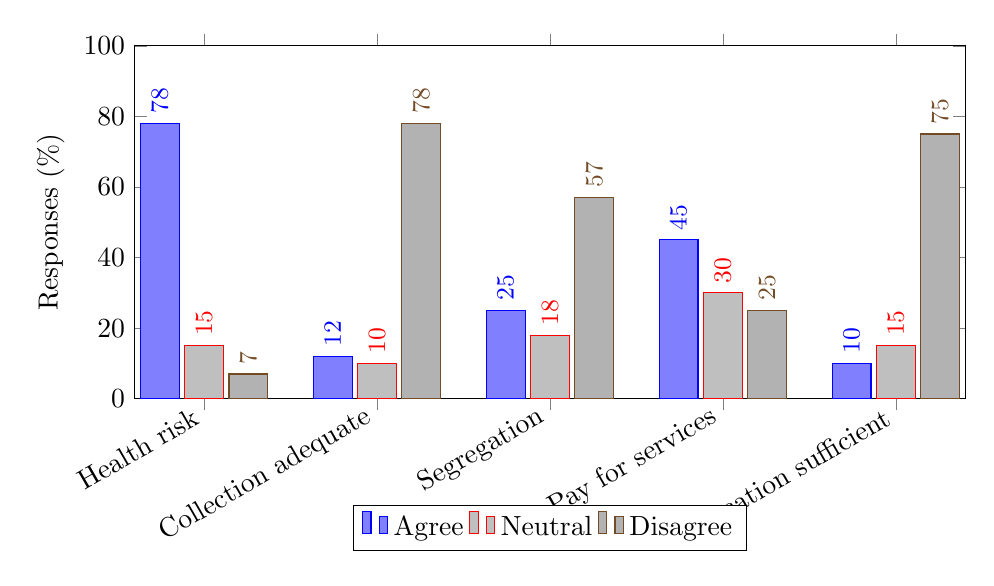
\begin{tikzpicture}
\begin{axis}[
    ybar,
    bar width=14pt,
    width=\textwidth,
    height=0.5\textwidth,
    ymin=0,
    ymax=100,
    ylabel={Responses (\%)},
    symbolic x coords={Health risk, Collection adequate, Segregation, Pay for services, Education sufficient},
    xtick=data,
    x tick label style={rotate=30, anchor=east},
    nodes near coords,
    nodes near coords style={font=\small, rotate=90, anchor=west},
    enlarge x limits=0.1,
    legend style={at={(0.5,-0.3)},anchor=north,legend columns=-1},
]
\addplot+[fill=blue!50] coordinates {(Health risk,78) (Collection adequate,12) (Segregation,25) (Pay for services,45) (Education sufficient,10)};
\addplot+[fill=gray!50] coordinates {(Health risk,15) (Collection adequate,10) (Segregation,18) (Pay for services,30) (Education sufficient,15)};
\addplot+[fill=black!30] coordinates {(Health risk,7) (Collection adequate,78) (Segregation,57) (Pay for services,25) (Education sufficient,75)};
\legend{Agree, Neutral, Disagree}
\end{axis}
\end{tikzpicture}
\caption{Community awareness and attitudes towards solid waste management.}
\label{fig:awareness}
\end{figure}

